\SetPicSubDir{ch-methodology}
\SetExpSubDir{ch-methodology}

\chapter{Methodology}
\label{methodology}
This chapter explains the methodology employed in our study, which includes the solvers, datasets, and evaluation metrics.

\section{Solvers}
We will employ five QUBO solvers for the study:
\begin{enumerate}
    \item D-Wave Quantum Annealing
    \item Neural Network Quantum States (NNQS)
    \item Quantum Approximate Optimization Algorithm (QAOA)
    \item GUROBI Optimizer
    \item Fixstars Amplify QUBO Solver
\end{enumerate}
The following sections will provide more information on the solvers.

\subsection{D-Wave Quantum Annealing}
We will use quantum annealers from D-Wave Systems, which produce the most popular commercially available quantum annealing hardware. The annealers are accessed with D-Wave's Solver API and use radio frequency superconducting quantum–interference device (rf-SQUID) qubits to represent spin variables during the annealing process \cite{b14}. External magnetic fields represent the linear interactions ($h$ terms), while couplers help entangle pairs of qubits to represent the interaction between qubits ($J$ terms). The qubits are arranged in the Pegasus graph topology shown in \autoref{pegasustopology} that allows up to 15 couplers per qubit \cite{b14}. 

\begin{figure}[!htb]
    \centering
    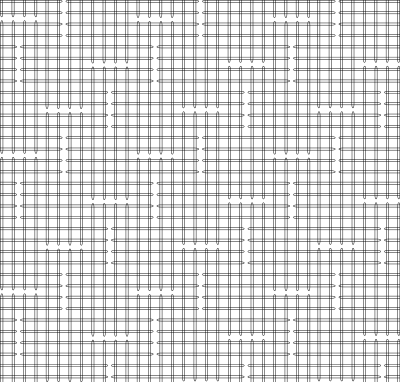
\includegraphics[width=0.4\linewidth]{images/pegasus_topology.png}
    \caption[A view of the D-Wave pegasus topology. Each line represents a qubit, and intersections represent available couplers. Each qubit can only be coupled to at most $15$ other qubits.]{A view of the D-Wave pegasus topology. Each line represents a qubit, and intersections represent available couplers. Each qubit can only be coupled to at most $15$ other qubits. ~\protect\cite{dwaveadvantage}}
    \label{pegasustopology}
\end{figure}

The experiments will be conducted with the D-Wave Advantage 4.1 QPU, which has up to 5640 qubits and 40484 couplers \cite{dwaveadvantage}. Given a target QUBO problem to solve, the process for using a D-Wave annealer is as follows:
\begin{enumerate}
    \item \textbf{Problem Definition} QUBO problem is first converted to its corresponding Ising model.
    \item \textbf{Minor Embedding} As the D-Wave quantum processing unit shown in \autoref{pegasustopology} is not fully connected, a single spin variable may need to be represented by multiple qubits called a \textit{chain}, which are forced to return the same value with large interaction terms \cite{b16}. The EmbeddingComposite class in the D-Wave library performs the embedding.
    \item \textbf{Programming} The parameters of the annealing process are set, which consists of the linear term for each qubit (with an external magnetic field acting on each qubit) and coupler strength (represents variable interaction between spins).
    \item \textbf{Initialization} The QPU is initialised in the ground state of the initial Hamiltonian, which is usually a superposition of all possible states.
    \item \textbf{Annealing} The system evolves with a time-varying Hamiltonian:
    \begin{equation}
        \label{eqn:dwavehamiltonian}
        4.
    \end{equation}
    where $s$ is the normalised anneal fraction and $A(s), B(s)$ are annealing functions shown in \autoref{dwaveannealing}. We will use the default annealing time of $20\mu s$. 
    \item \textbf{Readout of solution} The spin values of the qubits are measured and stored as a possible solution.
    \item \textbf{Resample} As finite-time quantum annealing does not guarantee optimality, we repeat the annealing and sampling process for $1000$ iterations and use the sample with the lowest energy as the candidate solution.
\end{enumerate}

\begin{figure}[htb!]
    \centering
    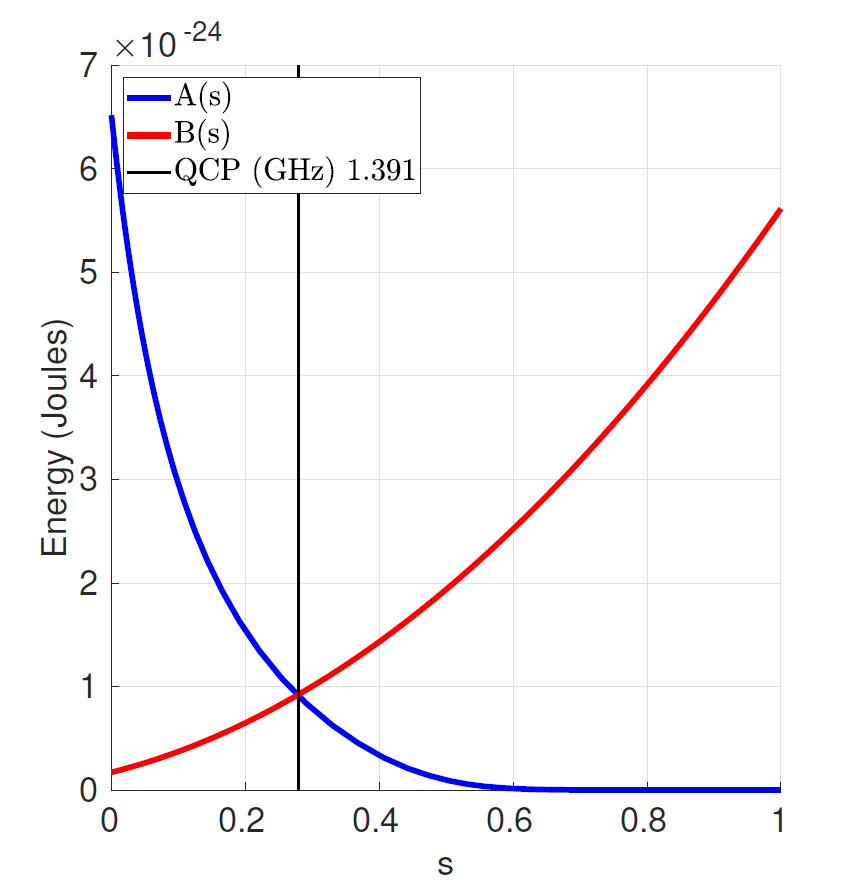
\includegraphics[width=0.5\linewidth]{images/dwave_annealing.png}
    \caption[Annealing functions $A(s)$ and $B(s)$ as a function of the normalised anneal fraction $s$. $A(s) >> B(s)$ when $s=0$ and $B(s) >> A(s)$ when $s=1$.]{Annealing functions $A(s)$ and $B(s)$ as a function of the normalised anneal fraction $s$. $A(s) >> B(s)$ when $s=0$ and $B(s) >> A(s)$ when $s=1$. ~\protect\cite{dwaveadvantage}}
    \label{dwaveannealing}
\end{figure}

\subsection{Neural-Network Quantum States}
We will adopt the Python library nqs\-tensorflow\footnote for implementing Neural-Network Quantum States \cite{b25}. The library uses Tensorflow to enable parallel execution on general-purpose graphics processing units for quicker sampling. We will use the Restricted Boltzmann Machine with $5n$ hidden nodes and the sigmoid activation function as the underlying architecture for the NNQS.

To solve a QUBO problem, the NNQS simulates the D-Wave quantum annealing process on a classical computer with a time-dependent Hamiltonian that follows \autoref{eqn:annealinghamiltonian}. Since the equations for $A(s)$ and $B(s)$ are unavailable, we employ a curve-fitting process to obtain analytical functions from the discrete points provided by D-Wave. The annealing functions used are:
\begin{gather}
    A(s) = 1.11e^{-7.06s} + -0.00569 \\
    B(s)= 0.680s^2 + 0.288s + 0.0305
    \label{fittedeq}
\end{gather}
The curve fitting process is detailed in \autoref{appendix:curvefitting}. The NNQS will be trained with a progressive training schedule that mimics the quantum annealing process and follows \autoref{alg:progressive}. $\hat{H}_c$ is the problem Hamiltonian and $\hat{H}_0$ is a Hamiltonian with linear biases as $1$ and no quadratic terms. The normalised anneal fraction $s$ is increased in small steps while the NNQS is trained to convergence, which simulates the slow change in the system Hamiltonian during quantum annealing. Like quantum annealing, the NNQS remains in the ground state throughout the training as it is trained to convergence.

\begin{algorithm}
    \begin{algorithmic}
    \Require Problem Hamiltonian $\hat{H}_c$
    \Ensure Trained NNQS
    \State Initialize NNQS with random weights;
    \For {$s \in [0.1, 1.0]$ step $0.1$}
    \State Set $H(s) \leftarrow A(s)\hat{H}_0 + B(s)\hat{H}_c$;
    \State Train NNQS on $H(s)$ until convergence or until epoch limit of $100$ is reached;
    \EndFor
    \end{algorithmic}
    \caption{NNQS Progressive Training}
    \label{alg:progressive}
\end{algorithm}

The training process of the NNQS involves updating the parameters, $\boldsymbol{\theta}$, with a Variational Monte Carlo approach to minimise the energy expectation value. The training algorithm is described as follows:
\begin{enumerate}
    \item Sample a set of $1000$ configurations $\mathbf{s}$ from the probability distribution defined by the NNQS, $\probP(s) = |\Psi(s;\theta)|^2$, with Gibbs sampling \autoref{samplingmethods}.
    \item Calculate an unbiased estimate of the energy expectation value with the average energy of the sampled configurations.
    \item Compute the gradients of the energy expectation value with respect to the NNQS parameters using backpropagation.
    \item Update the parameters with Root Mean Squared Propagation (RMSprop), a gradient-based optimiser, with a learning rate of $0.001$ \cite{rmsprop}.
    \item Repeat steps 1-4 for $1000$ iterations or until convergence is reached.
\end{enumerate}
The derivation of the gradients is detailed in the appendix of \cite{b20}. The candidate solution will be the best among the $1000$ configurations sampled from the final NNQS. All NNQS experiments were run on a 32 Core AMD 7543P Processor and an NVIDIA A100 40GB GPU with 500GB of RAM.

\subsection{Quantum Approximate Optimization Algorithm}
We will implement QAOA in Qiskit, an open-source software development kit for quantum computing, with $p=1$ using a backend hosted on the IBM Quantum Platform (IBMQ) \cite{b24}. We will utilise the IBMQ simulator, \texttt{ibmq\_qasm\_simulator}, a general-purpose simulator for quantum circuits that can handle up to 32 qubits. Even though IBMQ allows for access to quantum computers, it is limited by long wait times ($>5$ hours for each problem) and is infeasible for a benchmarking experiment. To measure the optimal performance of the QAOA algorithm, we will assume an ideal circuit without a quantum noise model. We will use the default mixing Hamiltonian of $\Hat{H}_0 = \sum_{i}\Hat{\sigma}_x^{(i)}$ and the Qiskit transpiler to optimise the decomposition of the operators into their individual parametrised quantum gates as shown in \autoref{qiskitcircuit} \cite{qiskittranspiler}.

 

The parameters $(\boldsymbol{\gamma}, \boldsymbol{\beta})$ are updated to minimise the energy expectation value. The training algorithm is described as follows:
\begin{enumerate}
    \item Initialise the circuit in the initial state $| + \rangle^{\otimes n}$ where each qubit is in a superposition state. Initialise $\gamma$ and $\beta$ with values sampled from a standard Gaussian normal distribution. 
    \item Construct the operators $U_C(\gamma), U_B(\beta)$ with $\gamma, \beta$, which consists of different quantum gates.
    \item Repeatedly sample the final states of the qubits and calculate an unbiased estimate of the energy expectation value as the average energy of the sampled configurations.
    \item Use a classical derivative-free optimiser Constrained Optimisation by Linear Approximation (COBYLA) to optimise the parameters $\gamma, \beta$ to minimise the energy expectation value.
    \item Repeat steps 2-4 for some iterations or until convergence is reached.
\end{enumerate}
We will repeatedly sample the final optimised circuit $1000$ times, and the candidate solution will be chosen as the best solution among the sampled configurations. The QAOA solver is accessed with the IBM Quantum Qiskit Runtime API and is run on the IBMQ cloud servers.

\subsection{GUROBI Optimizer}
The GUROBI optimiser is a state-of-the-art classical commercial solver \cite{b26}. The GUROBI optimiser uses a branch and bound algorithm that first relaxes the integer constraint of the QUBO problem, then branches into subproblems based on variables that violate the constraints. As the GUROBI optimiser supports QUBO problems, we construct the QUBO matrix directly and run the optimiser locally for $10$ minutes for each input problem. If the optimiser finishes before the cutoff, the candidate solution is guaranteed to be the optimal configuration. Otherwise, we would use the best solution within the cutoff time as the candidate solution.  All experiments were run on a 32 Core AMD 7543P Processor using Gurobi Optimizer version 10.0.3.

%All GUROBI experiments used the Gurobi Optimizer version 9.0.1 and were run on a local machine with an 8-core Apple M1 chip at 3.2GHz with 16GB of RAM.

\subsection{Fixstars Amplify QUBO Solver}
The Fixstars Amplify QUBO solver is a commercial simulated annealing-based QUBO solver that runs in parallel on GPUs on Fixstars' remote servers \cite{b12}. As the Fixstars solver supports QUBO problems, we submit the QUBO matrix using the Fixstars API and run the solver with the highest allowed time limit of $100$ seconds for each input problem.

\section{Benchmark datasets}
We use three randomly generated problem sets to benchmark our QUBO solvers: not-all-equal 3-satisfiability (NAE3SAT), max-cut, and the Sherrington-Kirkpatrick (SK) model. These problems were chosen as they are commonly used in QUBO experiments to represent NP-hard problems and are relatively straightforward to encode into QUBO form. The NAE3SAT and max-cut problem sets are macro benchmarks (application-based) to represent practical combinatorial optimisation problems. In contrast, the SK model problem set is a microbenchmark designed as a difficult QUBO problem set. Each problem set comprises problems of 13 sizes, ranging from $10$ to $300$\footnote{$n \in [10,15,20,25,30,35,50,75,100,150,200,250,300]$}. $20$ different random problems are generated\footnote{random seed is chosen to be from $0-19$} for each problem size for a total of $260$ problems per problem set. Each problem is first formulated in either the QUBO or Ising form, and the conversion between them follows \autoref{qubotoising} and \autoref{isingtoqubo}.

\subsection*{Not-all-equal 3-satisfiability (NAE3SAT)}
The NAE3SAT problem is a variant of the boolean satisfiability problem where each problem instance consists of $n$ boolean variables $(x_1, x_2, ..., x_n)$ and $m$ clauses that each combine three literals, which can be a variable or its negation. The objective is to find an assignment of boolean values such that the three values in each clause are not all the same, i.e., each clause has at least one true and one false value. We generate random NAE3SAT problems with $\rho = \frac{m}{n} = 2.1$, where NAE3SAT problems are known to transition from being satisfiable to unsatisfiable \cite{nae3sattransition}, using the random\_nae3sat generator from the dimod Python library, which uniformly samples 3-variable clauses with replacement \cite{dimodrandomnae3sat}. 

To convert a NAE3SAT problem into an Ising problem, we represent each boolean variable as a spin variable and turn each clause into a Hamiltonian term. For example, the clause $(x_1, x_2, \neg x_3)$, becomes the Hamiltonian term $H(s_1, s_2, s_3) = s_1 \cdot s_2 + s_2 \cdot (-s_3) + s_1 \cdot (-s_3)$ which has a value of $3$ when $x_1=x_2=\neg x_3$ and $-1$ otherwise. The final Hamiltonian $\Hat{H}_c$ is simply a sum of the individual Hamiltonian terms for each clause.

\subsection*{Max-cut}
The max-cut problem aims to find a partition of the vertices of a graph $G = (V, E)$ into $V_0, V_1$ with $V = V_0 \cup V_1$ and $V_0 \cap V_1 = \emptyset$, to maximise the number of edges crossing $V_0$ and $V_1$. We will use the Erdos-Renyi model to generate random graphs with $n$ vertices and a probability $p=0.25$ for each edge to be in $E$.

To convert a max-cut problem into a QUBO problem, we represent the assignment of each vertex as a binary variable ($x_v = i$ if $x \in V_i$) and use the objective function $f(\mathbf{x}) = \sum_{e = (u, v) \in E} -x_u - x_v + 2x_u x_v$, where each term has a value of $-1$ when $x_u  \neq x_v$ and $0$ otherwise. When the cut value is maximised, $f(\mathbf{x})$ is minimised. 

\subsection*{Sherrington-Kirkpatrick (SK) model}
The Sherrington Kirkpatrick (SK) model is an Ising problem with a random Hamiltonian of the form $\hat{H}_c = \frac{1}{\sqrt{n}} \sum_{1 \leq i < j \leq n} J_{ij}s_i s_j$
where $J_{ij} \sim \mathcal{N}(0,1)$ are independent standard Gaussian variables. The energy landscape of the SK model is complex as it has exponentially many local minima with a unique global minimum separated by high energy barriers \cite{skmodel}. This many-valley structure implies that finding the exact solution of the model is challenging. We generate random Gaussian variables with a random normal generator from the NumPy Python library.

%Parisi [6] provides a formula (for proof, see [7]) that, when numerically evaluated [8, 9, 1], shows for typical instances,
%\begin{equation*}
%    \lim_{n\rightarrow \infty} \argmin \frac{E}{n} = -0.763166...
%\end{equation*}
%(get from this paper https://quantum-journal.org/papers/q-2022-07-07-759/pdf/)

%\subsection*{Quantum Critical Points}
%get rid of linear term
%J terms are 1
%Ising model has no linear term
%QCP is A(s)/2 = +-B(s)/2 * J magnitude is the same.
%harder for Dwave to solve, jump to excited state
%finite infinite approximating

%We plan to use a subset of the 3296 QUBO problems provided by MQLib as our benchmark dataset. These problems are publicly accessible and contain both "real-world problem instances" and randomly generated problems \cite{b12}. The dataset also contains problems of various sizes and densities. The exact benchmark dataset will be determined after further testing to determine the input limits of each solver. Each QUBO problem will first be converted into an Ising model problem and then passed to each solver.

\section{Performance evaluation}
We use two metrics to evaluate the performance of the solvers, which are calculated separately for each problem type and size:
\begin{enumerate}
    \item The success probability, which is the probability of finding a solution with the lowest energy among all solutions found by the $5$ solvers. Since we are generating $20$ problems of each type and size, the success probability for each solver is:
    \begin{equation}
        \Bar{p} = \frac{\text{number of lowest energy solutions found}}{20}
    \end{equation}
    \item The average normalised energy, used in \cite{b34}, which is:
    \begin{equation}
        \Bar{r}_{solver} =  \frac{1}{20} \sum_{i = 1}^{20} \frac{E^i_{max} - E^i_{solver}}{E^i_{max} - E^i_{min}}
    \end{equation}
    where $E^i_{max}$ and $E^i_{min}$ are the energies of the worst and best solutions found by all solvers for problem $i$, and $E^i_{solver}$ is the energy that the solver found for problem $i$. Note that if a solver finds the best solution, it gets a normalised energy of $1$; if it finds the worst solution, it gets a normalised energy of $0$. All solvers get a normalised energy of $1$ if all solutions have the same energy.
\end{enumerate}
The average normalised energy measures the quality of the solutions produced by the solvers, while the success probability measures the solvers' ability to find the best solution.